\chapter{Background \& Objectives}

\section{Problem Description}

The Travelling Salesperson Problem (TSP) is tasked with solving the problem "Given a list of cities and the distances between each city what is the shortest possible route that visits each city once and then returns to the origin city". This shortest route is called a Hamiltonian Cycle and has many applications such as in the fields of logistics, route planning and manufacturing\cite{acobook}. Dantzig, Fulkerson and Johnson were the first people to attempt to solve TSPs through the use of branch and bound\cite{dantzig1954solution}, the time taken to solve TSPs through this method was too high to be practical so since then TSPs have attempted to be solved through the use of many algorithms.

Every method to solve TSPs has a limit on the size of problems that it can solve because it would simply take too long to solve problems above a given size. My project is a way of solving TSPs through the use of clustering and an Ant Colony Optimisation (ACO) Algorithm. ACO is a probabilistic technique that is based off how ants work in nature, figure \ref{fig:aco_pheremone_example} shows an example of how the path of ants change as pheromone gets deposited.

\begin{figure}
    \centering
    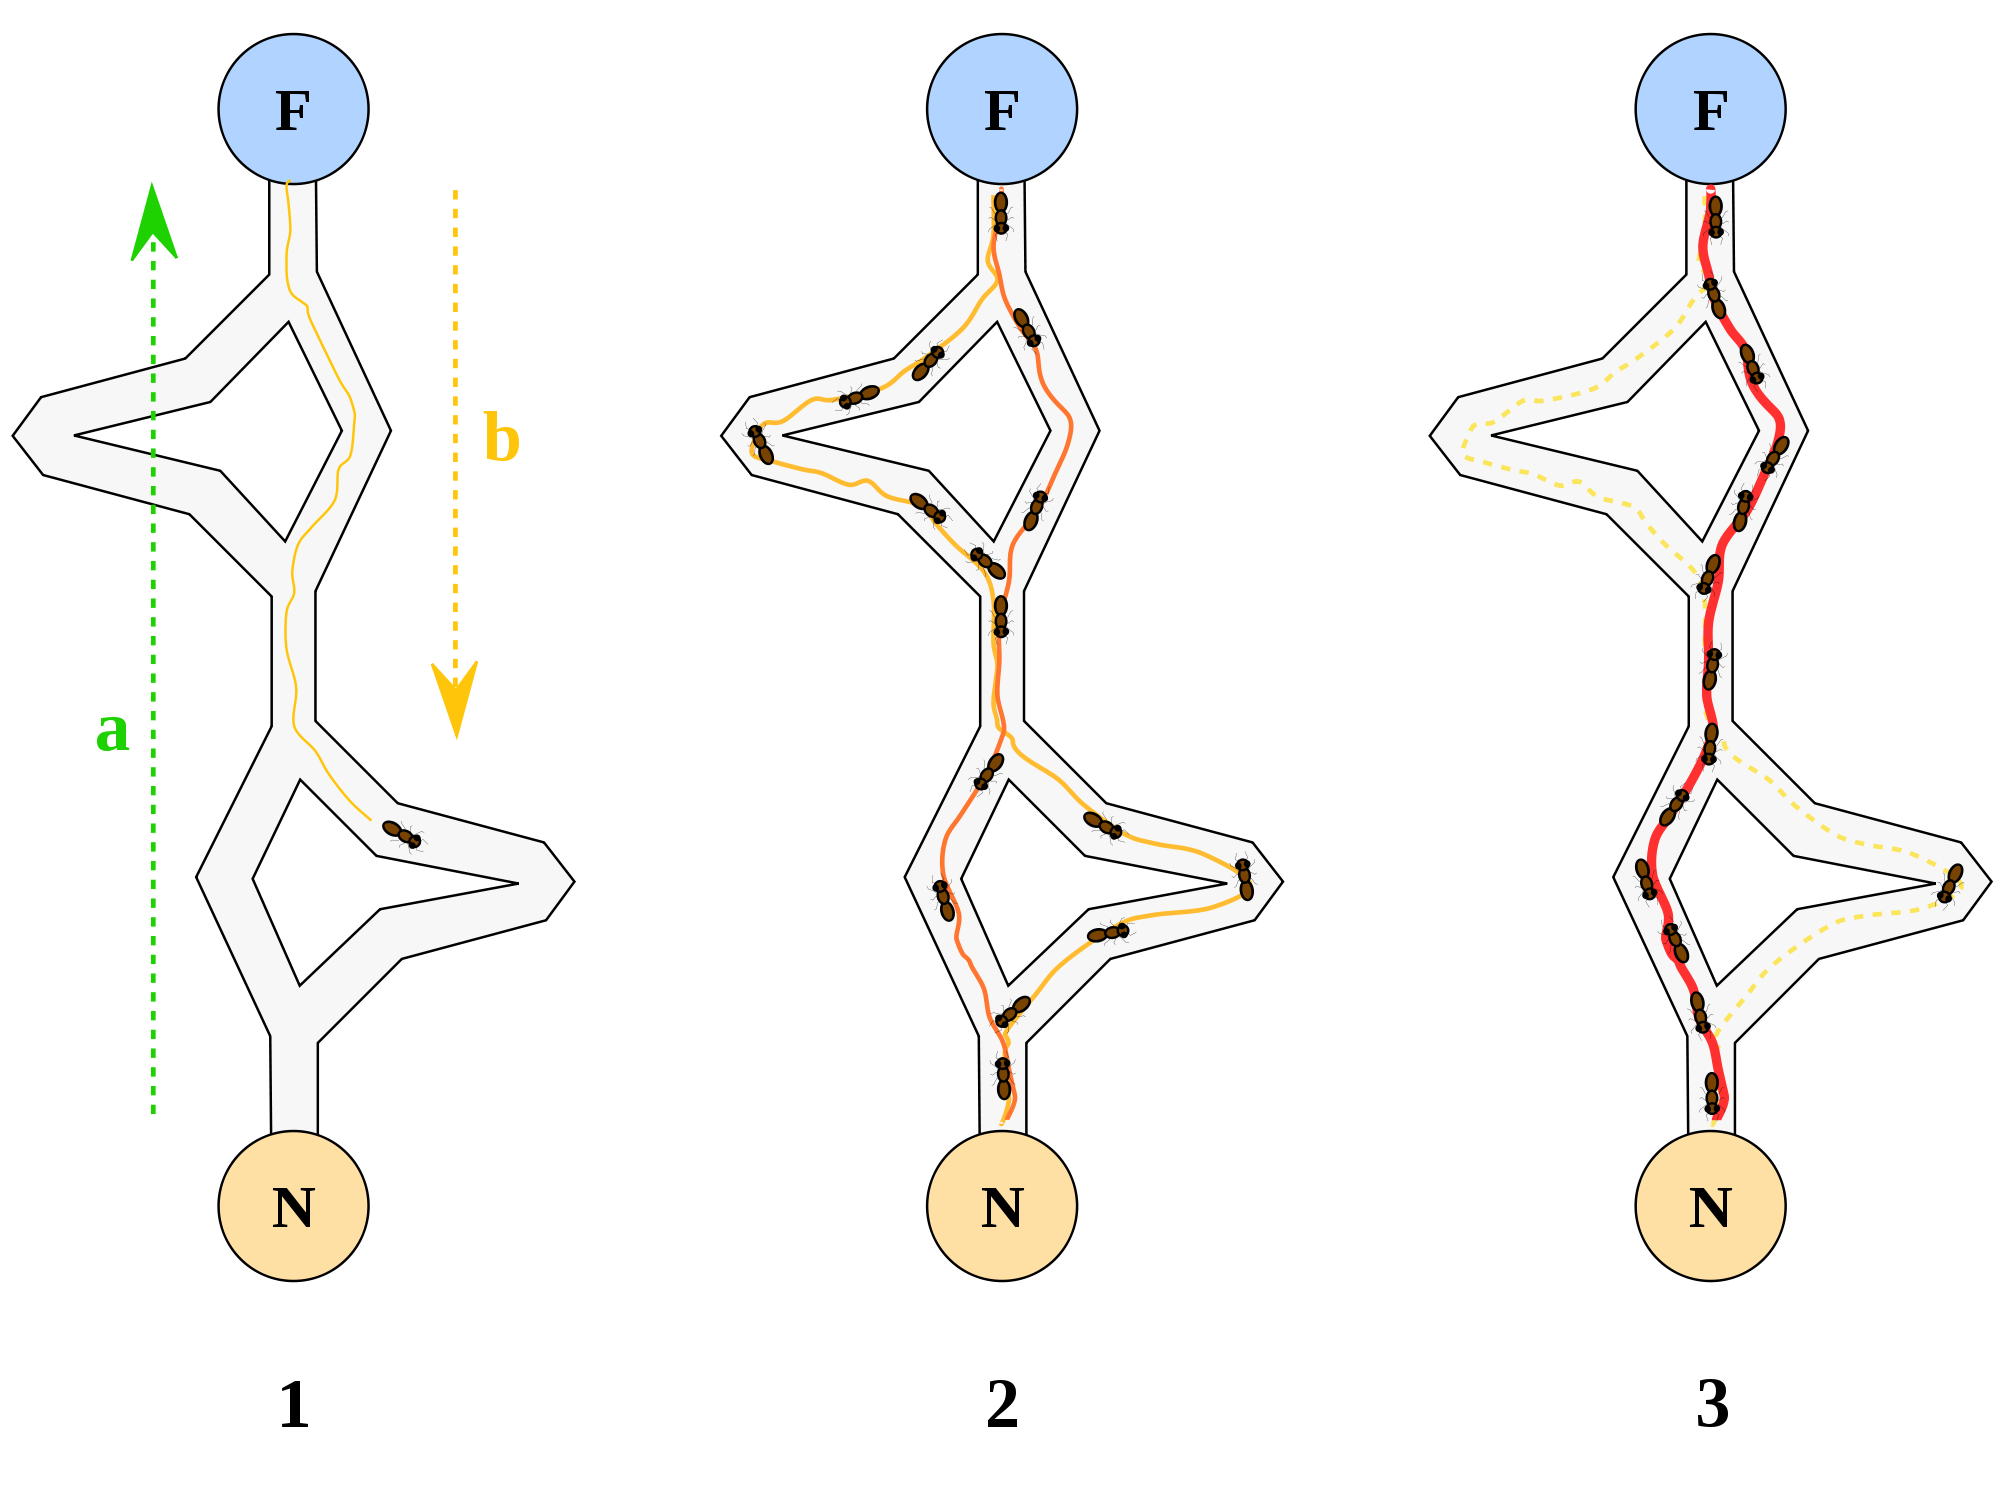
\includegraphics[width=\textwidth]{Project Report/LaTeX Template/figures/aco_pheremone_demo.png}
    \caption{Figure showing how in nature ants deposit pheromone and change their paths based on the pheromone from other ants. The Ants choose a path based on the pheromone that has been deposited but there is also a random chance that the ant will choose a different route, this is what allows ACO to change routes and find a better solution.}
    \label{fig:aco_pheremone_example}
\end{figure}

There are many freely available data sets of TSPs I have used the ones provided by The University of Waterloo\cite{tsp_test_data_2009} these are all of varying sizes and complexity and are provided in the common TSPLIB95 format, they also all have their optimal solutions noted so that easy comparisons can be made and so I can see how my algorithm performs. This TSP data is split into two main categories National and VLSI, National test data is based on cities on a map and range in size from 29 nodes to 71,000 nodes, VSLI data is based on solder points in circuit boards. These two types of problems look very different and will require different types of clustering algorithms to properly solve. Figure \ref{fig:vlsi_tsp_data} shows VLSI test data and figure \ref{fig:world_tsp_data} shows an example of a world TSP problem.

\begin{figure}
    \centering
    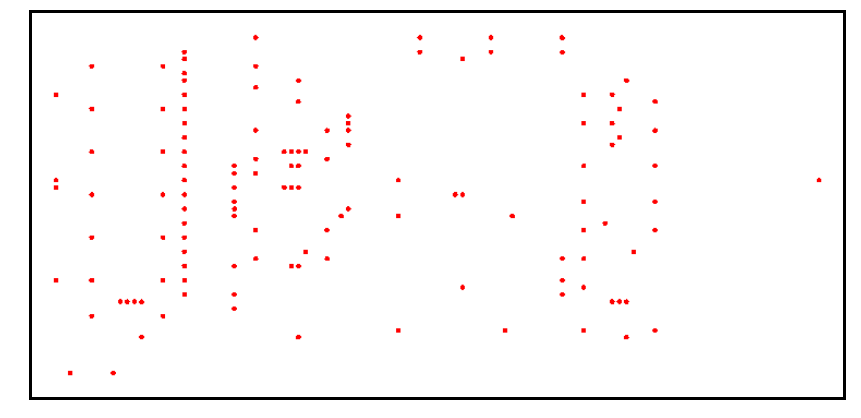
\includegraphics[width=\textwidth]{Project Report/LaTeX Template/figures/vlsi_xqf131_tsp_data.png}
    \caption{Figure showing VLSI TSP test data, the nodes in this problem form in lines and therefore the clusters will need to extend and form into lines in order to get the most optimal soution. This problem came from \cite{xqf131_tsp_instance}.}
    \label{fig:vlsi_tsp_data}
\end{figure}

\begin{figure}
    \centering
    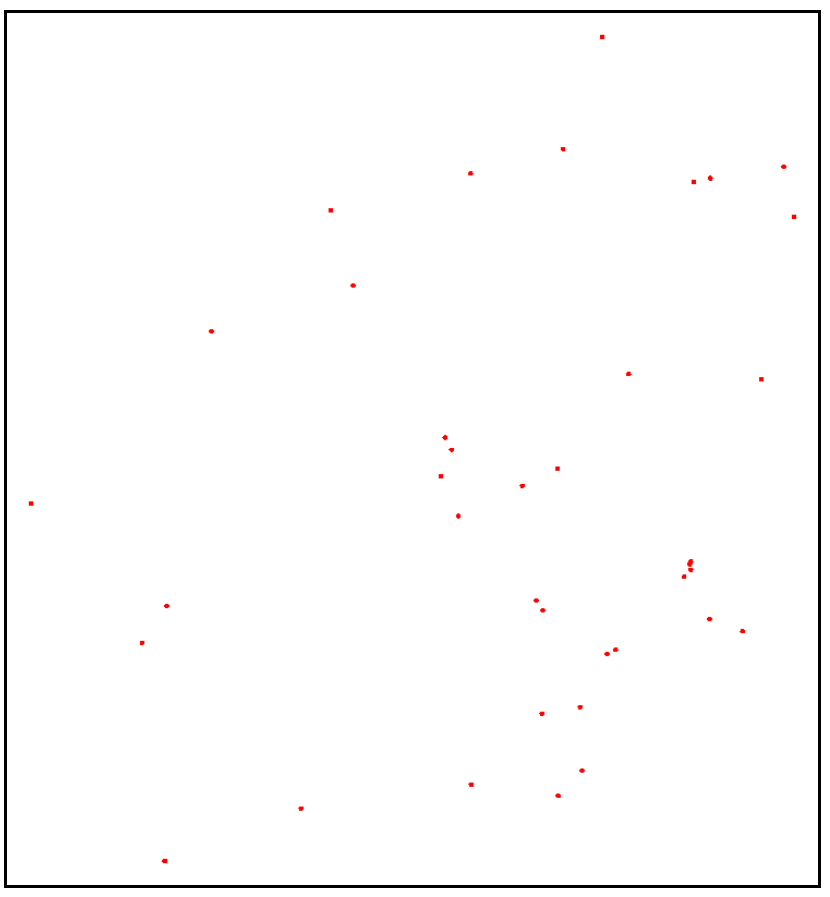
\includegraphics[width=\textwidth]{Project Report/LaTeX Template/figures/world_dj38_tsp_data.png}
    \caption{Figure showing world TSP test data, the nodes form like cities on a map. This example is based on 38 cities from Djibouti. This problem came from \cite{dj38_tsp_instance}.}
    \label{fig:world_tsp_data}
\end{figure}

\section{Background}
My motivation for this project was based around my interest in Algorithms and finding new approaches to solve challenging problems, In 1991 ACO was first applied to solve TSPs\cite{dorigo1991distributed} this algorithm was called "Ant System" and was tested on several TSPs. It was able to solve TSPs of small sizes but didn't perform as well in solving larger problems. ACO is not efficient at finding the solution for large problems because its run time is to high, it's possible to tune the parameters of the algorithm such as reducing the number of iterations it will perform however doing this could mean that it finds a worse solution. 

ACO has several parameters you can tune; the number of iterations that it runs, the number of ants that are simulated, the amount of pheromone that is deposited, the amount of pheromone that evaporates each iteration, the weighting that the pheromone has on the ants decision, called the alpha value, and the weighting that the distance of the edge has on the ants decision, this is called the beta value. ACO algorithms make a choice between whether they will follow the pheromone deposits or change path and follow a heuristic, this is what the alpha and beta values are for. This allows the algorithm to be probabilistic and is what makes it improve upon its tours, however because of this probabilistic nature it can produce different tours on consecutive runs. If you have a high alpha value then the ant is more likely to follow the other ants that came before it, and if you have a high beta value then the ant is more likely to choose a route that has the lowest distance. There is a balance to be struck because going to the closest node does not always result in the best overall tour.

The main way to cut the run time of ACO is to cut down on the number of nodes. The run time of ACO is \[O(t\textsubscript{max}MN^2)\] where \[M=N/1.5\] and t\textsubscript{max} is the number of iterations, M is the number of ants and N is the number of nodes\cite{pang_chao-yang_ben-qiong_zhang_jie_wei_shan_zheng-chao_2014}. The run time is proportional to N\textsuperscript{2} so the only way to cut down the run time of the algorithm without compromising the quality of the solution is to cut down the number of nodes.

There are many different clustering algorithms available it is my goal to implement quite a few of them so that there is a choice and the different clustering algorithms can be analysed in respect to their effect on ACO. The Python library sci-kit learn\cite{scikit_learn_python_library} has implemented many different clustering algorithms\cite{scikit_clustering} and so I will be using that to do my clustering, I will choose a selection of these algorithms and should be able to compare them to see which ones perform better against ACO.

The tour that ACO produces may not be optimal because it didn't run for long enough or the parameters where not tuned correctly to fix this there is a local search algorithm called 2-opt that takes a tour created from a heuristic and attempts to improve it\cite{venhuis_2019} It improves the tour by reordering the nodes, it performs very well at removing paths in the tour that cross over each other but does not always find the optimal solution because it is bound to the tour that was found in the heuristic and simply finds the local optimum of this. 2-opt swaps two nodes to see if there is an improvement there are other versions called 2.5-opt or 3-opt that swap more nodes to try and find a bigger improvement. 

** TALK ABOUT THE TOUR IN EACH CLUSTER**
When traversing the clustered tour there will need to be a way of going from the global clustered tour to the local inside each cluster tour. To do this there will need to be nodes assigned on each cluster that are the entry and exit nodes and then a tour will have to be made in each cluster from the entry node to the exit node. To find this tour I will implement ways of finding the solution with ACO and through a greedy nearest neighbours approach.

\section{Analysis}

\subsection{The Current State of Solving TSPs with ACO and Clustering}
As I've previously mentioned ACO has been applied to TSP many times before but this has mostly centred around using just ACO, in \cite{assesmentdiffacofortsp} different ACO algorithms are all put to work solving a particular TSP and assessed based on how quickly they take to run and how close to optimal their solution is. This paper considers five different ACO algorithms and offers a good comparison of how well suited these algorithms are to solve TSPs as well as offering good explanations of the types of ACO algorithms. 

Clustering has been used before as part of a solution to solve TSPs in \cite{clustering_with_local_search_heuristic}, in this study Clustering was used alongside a Genetic Algorithm and it showed that when using clustering the GA always finds a shorter solution for the TSP.

As briefly mentioned earlier \cite{pang_chao-yang_ben-qiong_zhang_jie_wei_shan_zheng-chao_2014} used ACO and clustering to solve TSPs and in their research they found that using clustering did speed up the ACO process they also created their own clustering algorithm the "Local Clustering Algorithm" which better expands to fit TSP data. 

\subsection{What I want to do}
There are many directions to take this project and things that I could discuss and do however because I've only got a few months to do this project I'm going to be limited in what I can do. I would like to mostly look at the interactions of ACO on solving TSPs and seeing how clustering affects this, the questions that I propose answering for this are;

\subsubsection{Does clustering allow ACO to be applied to larger problems.}
This question is about seeing how clustering impacts the run time of ACO and if clustering the data means that the run time is slower. To evaluate this question I will choose several pieces of TSP data of various sizes and run ACO and clustering with ACO over them. I will then evaluate the run times of these algorithms as well as seeing if there is an improvement in solution length. I will run this on TSP data that is of the world and VLSI types and I will use the same clustering algorithm and the same ACO parameters for each run. I will use different sized TSP data to see if how this effects the impact on run time as well.

When the tour inside each cluster is calculated I will have a run that uses the ACO approach and another that uses the greedy nearest neighbours approach.


\subsubsection{To what effect do different clustering algorithms have on the quality and run time of the solution.}

This question is about seeing the change that clustering algorithms have on the solution. To run this experiment I will use the same ACO algorithm and parameters and then use different clustering algorithms to see if there is one that is particularly suited to use with TSP data. I will use TSP data of varying sizes as well as TSP that is of the VLSI type and the world type. To find the tour inside each cluster I will use both ACO and the greedy nearest neighbours approach. 


\subsubsection{When using 2-opt with ACO and clustering what effect do the clusters have on the overall solution, does 2-opt end up finding the same solution or nearly the same solution regardless of the clustering algorithm used.}

\subsubsection{What effect does varying the ACO parameters have on the solution.}

It would be interesting to see if I could create a new algorithm that can better deal with TSP data in 'Applying Data Clustering Feature to Speed Up Ant Colony Optimization'\cite{pang_chao-yang_ben-qiong_zhang_jie_wei_shan_zheng-chao_2014} they create a new local clustering algorithm that measures the direction in which TSP data extends. This allows the clusters to better form around TSP data which should result in a better overall solution. It would be nice to implement my own clustering solution but I feel in the time I have that this may not necessarily be possible. It might be possible to improve existing clustering methods to better account for TSP data or speed up the process of clustering. 

The best kind of clustering algorithms to use will be ones that can deal with data that doesn't belong to any specific cluster, in most TSP problems there will be data that will not neatly fit into any specific cluster and this should be able to be dealt with. 

In the time I have I will not be able to create an algorithm that can deal with massive TSPs that contain 10's of thousands of nodes or an algorithm that can necessarily find an optimal solution to every piece of data. I will instead focus on smaller problems and evaluating the results of these questions.